In order to support priorities and node partitioning, we extended the work queue
of each thread, as presented in Fig.~\ref{fig:implementation:vm_overview}, to
include two new pairs of queues: two doubly linked lists known as the
\emph{standard queue} and two min/max heaps known as the \emph{priority queue}.
The standard queue contains nodes without priorities and supports push into
tail, remove node from the head, remove arbitrary node, and remove first half of
nodes.  The priority queue contains nodes with priorities and is implemented as
a binary heap array.  It supports the following operations: push into the heap,
remove the \emph{min} node, remove an arbitrary node, remove half of the nodes
(vertical split), and priority update.  Operations for removing half of the
queue are implemented in order to support node stealing, while operations to
remove arbitrary nodes or update priority allows threads to change the priority
of nodes.  Table~\ref{fig:implementation:table_queue} shows the complexity of
queue operations and compares the standard queue against the priority queue.
Except for the remove half operation, priority queue operations are more
expensive.

\begin{table}[h]
   \begin{tabular}{| c | c | c |}
      \hline
      \textbf{Operation} & \textbf{Standard queue} & \textbf{Priority Queue} \\
      \hline
      Push & $\mathcal{O}(1)$ & $\mathcal{O}(\log{N})$ \\ \hline
      Pop & $\mathcal{O}(1)$ & $\mathcal{O}(\log{N})$ \\ \hline
      Remove & $\mathcal{O}(1)$ & $\mathcal{O}(\log{N})$ \\ \hline
      Remove Half & $\mathcal{O}(N)$ & $\mathcal{O}(\log{N})$ \\ \hline
      Priority Update & - & $\mathcal{O}(\log{N})$ \\ \hline
   \end{tabular}
   \caption{Complexity of queue operations for both the standard
      queue and the priority queue.}
   \label{fig:implementation:table_queue}
\end{table}

\begin{figure*}[t]
\centering
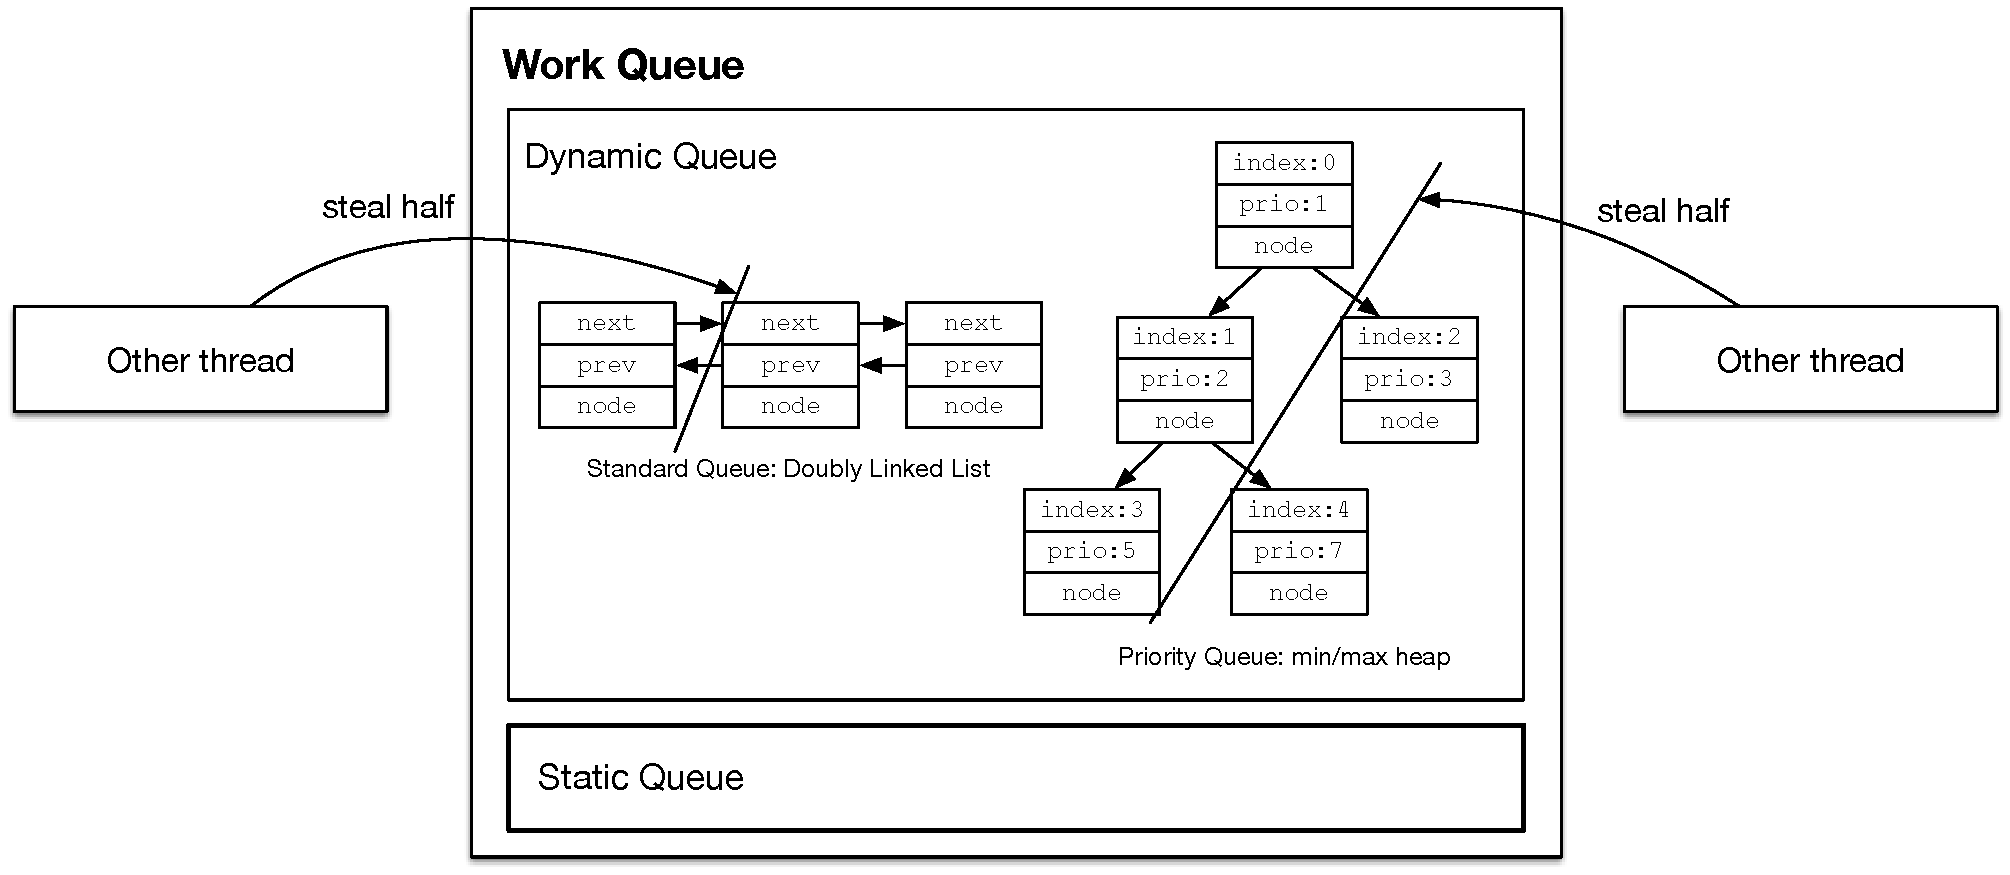
\includegraphics[width=0.95\textwidth]{figures/implementation/work_queue.pdf}
\caption{Thread's work queue and its interaction with other threads: the dynamic queue contains nodes that can be
   stolen while the static queue contains nodes that cannot be stolen. Both
   queues are implemented with one standard queue and one priority queue.}
\label{fig:implementation:work_queue}
\end{figure*}

The \texttt{next} and \texttt{prev} pointers of the standard queue are part of
the node structure in order to save space. These pointers are also used in the
priority queue but for storing the current priority and the index in the binary
heap array. Both the standard and priority queue are implemented as a pair of
queues. This first queue of each pair is a \emph{static queue} which contains
nodes that cannot be stolen and the second queue is the \emph{dynamic queue}
which contains nodes which can be stolen by other threads.
Figure~\ref{fig:implementation:work_queue} presents an overview of the two pairs
of queues and how the remove half operations are implemented in both queues in
order to support node stealing.  In the regular queue, the first $n/2$ elements
are removed from the front of the list and, in the priority queue, the binary
heap is split vertically for improved distribution of priorities.

Remember that to minimize inter-thread communication, node priorities are
implemented at the thread level, i.e., when a thread picks the highest priority
node from the priority queue, it picks the highest priority node from its
subgraph of nodes and not the highest priority node from the whole graph.

\subsection{Node State Machine}\label{sec:node_state_machine}

To accommodate the new coordination facilities, we added a new node state to the
state machine presented previously in Fig.~\ref{fig:local:node_states}.
Figure~\ref{fig:implementation:node_states} reviews the new set of states of
the state machine.

\begin{itemize}
   \item \textbf{running}: The node is deriving rules.
   \item \textbf{inactive}: The node is inactive, i.e., it has no new facts and
      it is not in any
   queue for processing.
   \item \textbf{active}: The node has new facts and it is in some queue waiting
   to be processed.
   \item \textbf{stealing}: The node has just been stolen and it is in the process of being
   moved to another thread.
   \item \textbf{coordinating}: The node moves from one queue to another or
      inside the priority queue when changing its priority.
\end{itemize}

\begin{figure}[ht]
   \centering
   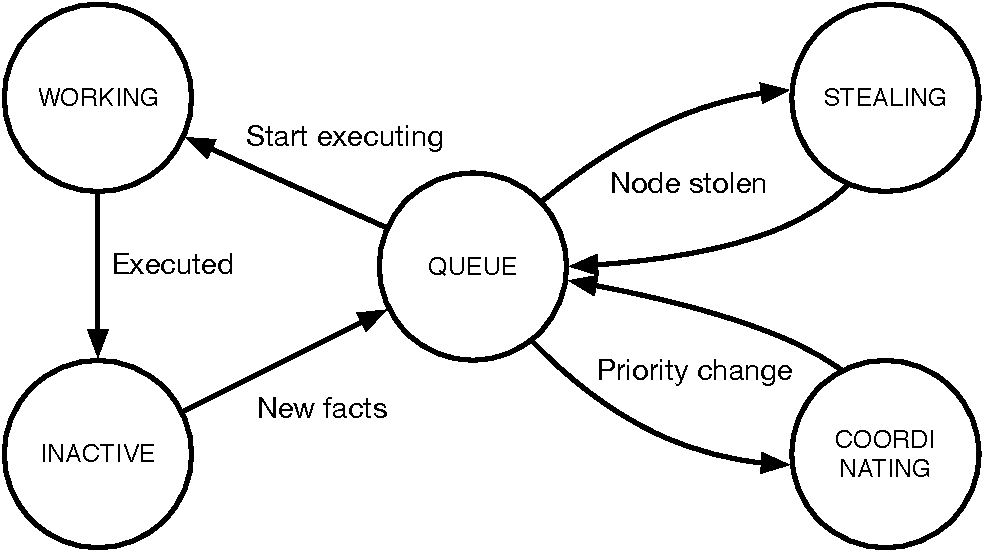
\includegraphics[width=0.55\textwidth]{figures/implementation/node_states.pdf}
   \caption{Node state machine extended with the new \textbf{coordinating}
   state.}
   \label{fig:implementation:node_states}
\end{figure}

\subsection{Coordination Instructions}\label{section:coordination:coord_instrs}

Coordination facts are implemented as API calls to the virtual machine which
implement the appropriate operations. Sensing facts read information about the
state of the virtual machine while action facts lock and update the appropriate
underlying data structures such as the node data structure or the thread's
queues.

When a thread $T_1$ performs coordination operations to a node owned by a thread
$T_2$, it needs to synchronize with $T_2$ and for that the \emph{State Lock} in
the target node needs to be acquired. Optionally, we may need to also lock the
queues of the thread $T_2$ if the priority is being updated or the queues of
thread $T_1$, if the node is moving to thread $T_1$. Note that both the standard
queue and priority queue have separate locks in order to allow concurrent
manipulation of the two data structures.

For the coordination facts \code{set-priority} and \code{add-priority}, when
multiple operations are directed to the same node during a single node
execution, we coalesce the multiple operations into a single operation.  As an
example, if a node derives two \code{set-priority} facts that change the
priority of node \code{@1} to \code{1} and \code{2}, the virtual machine
coalesces the two instructions into a single \code{set-priority} that is applied
with value \code{2} (the higher priority) after all the candidate rules of the
node are executed. The reason for this optimization is that nodes may be
executed several times and in short bursts during the lifetime of the program,
therefore immediately applying each and every coordination instruction is not
cost effective. We aim to reduce the amount of locking and movement of nodes
inside the queues due to priority updates.
